\documentclass[]{scrartcl}

%opening
\title{March Madness}
\author{Alexander Van Roijen, Rocco Bavuso, Molly Clark}
\usepackage[margin=1.0in]{geometry}
\usepackage{color}
\usepackage{times}
\usepackage[pdftex]{hyperref}

\newcommand{\fillin}[1]{\textcolor{red}{\textsc{#1}}}


\setlength{\parindent}{0in}
\setlength{\parskip}{2ex}
\renewcommand{\baselinestretch}{1.0}

\usepackage{graphicx}
\usepackage{caption}
\usepackage{float}

\begin{document}

\maketitle

\begin{abstract}
\begin{center}
\noindent This report analyzes what plays into the determination of March Madness seeding. We are taking a look at data from multiple past seasons of play, data from past tournaments, and at winners from the past to see if there is anything specific that points to the way teams are seeded within the tournament.
\end{center}
\end{abstract}

\section*{Introduction}
March Madness is an annual NCAA division 1 basketball tournament. The tournament occurs in the month of March, earning its name. There are 64 teams in the tournament each year, seeded into 4 Regions that each contain 16 teams. We will be taking a look at how these seeds are determined. The teams then play bracket-style and are eliminated game by game until one team reigns champion.\\

\noindent
We obtained our data from kaggle.com, and have broken the data up into three overarching sections: Regular Season Data, Tournament Data, and Seasons and Regions. We intend to analyze the data in each of these sections to see what affects a team's seeding within the tournament.

\section*{Data Summary}
From Kaggle's website, we downloaded a data set that gave us a look at the teams who qualified for the March Madness tournament in the past ~30 years. Each team is assigned a four digit code that is consistent from season to season and data set to data set. This allows us to easily manipulate and analyze the data across the different files.\\

\noindent
We began by looking at the data that has been collected season to season and follow up by looking at the data from previous tournaments and regional and past seed data to see which factors effect a team's chances of winning.\\

\noindent
Throughout this report, let the following be universally true:\\
{\textbf {Field Goals:}} defined as any shot that is made in the game and is worth 2 points (within the 3 point line, not a free throw)\\
{\textbf {Three Pointers:}} defined as any shot that is made in the game and is worth 3 points (outside the 3 point line, from any place)\\
{\textbf {Free Throws:}} defined as any shot that is made in the game and is worth 1 point (shot after being fouled in any form, from the free throw line)\\
{\textbf {Assist:}} defined as a pass to another player who then immediately scores\\
{\textbf {Rebound:}} defined as a play in which a player grabs the ball, which bounced off of either the rim or backboard on an attempted shot. For this paper, we include offensive and defensive rebounds\\
{\textbf {Turnovers:}} defined as any action that results in the loss of basketball. (an action that gives the basketball to the other team not including a failed shot attempt)\\
{\textbf {Steals:}} defined as a defensive play in which a player steals the basketball from an opposing player\\
{\textbf {Block:}} defined as a defensive play in which a player deflects an opposing shot attempt before it reaches the basket\\
{\textbf {Personal Fouls:}} defined as an action that results in either a loss of possession or free throws for the other team\\
\subsection*{Regular Season Data}
Part of our analysis comes from regular season data of 71,241 NCAA Division 1 games from 2003 to 2016. The data available are game statistics of winning and losing teams, such as field goals made, rebounds, assists, etc. For this part of the analysis we wanted to determine particular characteristics of winning teams in the regular season visible on the stat sheet. This part was used to help determine what are the best predictors of a winning team, and thus the best predictors of a team advancing far into the tournament. In order to do so, we thought the ideal comparison would be winning team statistics compared to losing team statistics. We computed this difference for the following statistics: field goal, three point, and free throw percentage, rebounds, assists, turnovers, steals, personal fouls, and blocks. The first three statistics are percentages while the rest are averages per game.
\subsection*{Tournament Data}
With the Regular Season Data, we included data that came specifically from the March Madness Tournament. This data was pulled out of tournaments from 1985 to 2016 and includes information on both winning and losing teams throughout the tournament. The stats that are available to us through this data set include attempted and made field goals, three pointers, and free throws, as well as the seeds and slots of the teams. We analyze the differing percentages of made shots between winning and losing teams to see what may make a difference in a team's ability to win more tournament games. We took a look at past seed placement with the season and tournament data to determine potential placement in coming tournaments.
\subsection*{History of Success}

Temporal data is obviously very important when trying to do analysis and prediction of team performance. It is very true that expectations of each team make all the difference, and even more so, how well each team lives up to those expectations. Looking at previous records give us an indication of well we expect them to do in the future. For example, as we will see, schools like UNC and Duke tend to preform very well each year, and thus we can expect those teams to preform well in the tournament. This section aims to tabulate this History of Success and see how much it may influence seeding and tournament performance.
\section*{Pre-Analysis}
\subsection*{Regular Season Data}
\begin{figure}[H]
	\centering
	\includegraphics[scale=.6]{SeasonShotPercent.png}
\end{figure}
These boxplots represent the differences in field goal, three point, and free throw percentages amongst winning and losing teams. Clearly the winning teams on average have higher percentages. The following are the averages:
\begin{verbatim}
            Winners    Losers
Field Goal  0.4737919 0.4007075
Three Point 0.3811237 0.3071846
Free Throw  0.7066836 0.6701483
\end{verbatim}
The differences in three point and field goal percentages are very critical. A basketball game is often decided by a few points, these percent differences equate to stark point differentials over time.
\begin{figure}[H]
	\centering
	\includegraphics[scale=.6]{GameAverages.png}
\end{figure}
\begin{figure}[H]
	\centering
	\includegraphics[scale=.6]{GameAverages2.png}
\end{figure}
The previous two boxplots demonstrate per game averages for important offensive and defensive stats. Some are more significant than others, as we can more easily see by the averages:
\begin{verbatim}
               Winners    Losers
Rebounds       36.460100 32.643099
Assists        14.677138 11.394478
Turnovers      13.118457 14.481029
Steals          7.111551  6.082340
Blocks          3.839110  2.868587
Personal Fouls 17.477099 19.867829
\end{verbatim}
The only particularly noticeable differences are among rebound and assists. This is intuitive as these actions occur much more frequently during the course of a basketball game. Based on these results, we would not include turnovers, steals, blocks, and personal fouls into our final analysis. The difference between winning and losing teams for these statistics is so marginal theres reason to believe these factors are not as critical as others in determining a teams chances of progressing deep into the tournament.
\subsection*{Checking Parameters for Normality}
In order to test potential parameters for normality, we look at the QQ-plots. For field goal percentage, three point percentage, rebounds per game, and assists per game. Due to the large sample size, over 140,000, we do not anticiapte having issues due to the Central Limit Theorem.  
\begin{figure}[H]
	\centering
	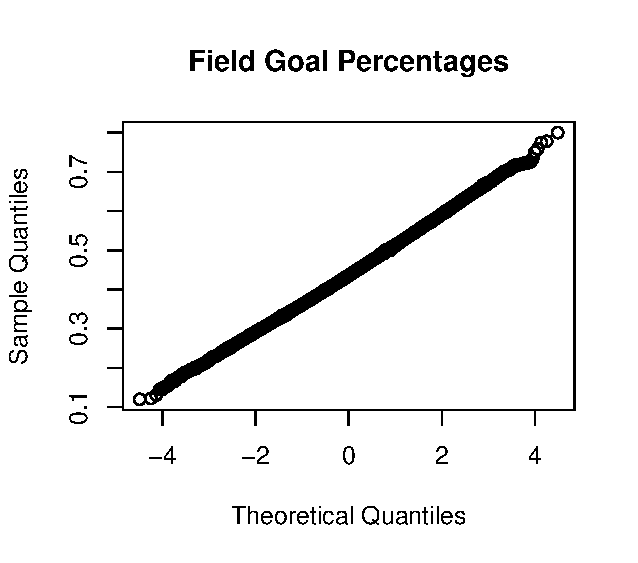
\includegraphics[scale=.6]{FGnorm.pdf}
	\includegraphics[scale=.6]{3pnorm.pdf}
	\includegraphics[scale=.6]{rbnorm.pdf}
	\includegraphics[scale=.6]{assnorm.pdf}
\end{figure}
The only parameter of concern here is the tails of the three point percentage. The minimum and maximum values of this value are 0 and 1, respectively. The issue here lies in the fact that there are several data points with these minimum and maximum values, but there is a gap of values just above the minimum and just below the maximum. For example, for a team to shoot 1 percent on three pointers, the team would have to only hit 1 and attempt 100. This is not plausible. However, a team can only attempt 5 three points and miss all of them, giving them a three point percentage of 0. The same analysis can be made for the maximum value. 
\subsection*{Tournament Data}
\begin{figure}[H]
	\centering
	\includegraphics[scale=.6]{TourneyShotPercent.png}
\end{figure}
This analysis stems from the detailed tournament data that was outlined on kaggle. Boxplots are used to show the general trends in data from the past tournaments. The comparison is visible due to the color differentiation, with blue representing the winning teams' data and red representing the losing teams' data. In general, it is pretty plain to see that winning teams, on average, have higher shooting percentages across the board. There clearly are some outliers in this data set, which we will need to investigate further as we move forward to ensure that it is not affecting our outcome.
\begin{figure}[H]
	\centering
	\includegraphics[scale=.6]{GameScores.png}
\end{figure}
This figure shows the average scores in tournament games differentiated by whether the teams win or lose. As suspected, on average, the winning teams score more per game. This boxplot does visualize the data easily though, and it allows us to pick out any potential outliers that may affect our future analysis.
\subsection*{History Of Success}
As we all know from our sporting careers, certain teams we have watched, played against, or played with can have a history of success. Meaning, despite the ups and downs of each team from year to year, some teams are known to succeed. The same goes with college basketball, there are top performers.
\begin{figure}[H]
	\centering
	\includegraphics[scale=.75]{XConfLeader.pdf}
	\caption[leaders]{Best teams in the X Region by reporting the teams only entering within the top 4 seeds from the years 1985-2015. We see that teams that get the number one seed tend to stay within the top four }
	\label{rVals}
\end{figure}
To specify, the "X" conference is a region up to change with each season. In general, X is usually the West, Midwest, Southeast, or the South. "W" almost always represents the East, and so on for Y and Z. 
\begin{figure}[H]
	\centering
	\includegraphics[scale=.75]{overLeaders.pdf}
	\caption[overallLeaders]{Best teams over all regions. This shows the upper echelon of basketball teams and the many others that try and compete}
	\label{rVals}
\end{figure}
We can also look at how these teams tend to actually preform in the tournaments by seeing how many games they have played over all these years.
\begin{figure}[H]
	\centering
	\includegraphics[scale=.75]{HistOfSuccess2.pdf}
	\caption[HistOfSuccess]{This shows the teams with the most appearances in the march madness tournament. The more appearances illustrate they make it further in the tournament than others}
	\label{rVals}
\end{figure}

Overall, this is to show that the parameters of $\beta_s$, or seed, and $\beta_a$, appearances, of a teams history is indicative of their future success. The remaining region seed frequencies can be found in the appendix
\section*{Proposed Model}
	\[
	Y_{daynum} = \beta_0 + \beta_{conf} + \beta_{fgp} +\beta_{tpp} + \beta_{ass} + \beta_{rb} + \beta_{app} + \epsilon
	\]
	\begin{itemize}
	\item The response variable, daynum, signifies what day of the year the last game is played for each team. This is a good measure of two things: If a team makes the tournament and how far that team advances.
		\item Conf refers to the conference the team plays in. Different conferences have vastly different quality of teams.
	\item 	Fgp refers to field goal percentage - calculated by field goals made divided by field goals attempted.
	\item 	Tpp refers to three point shooting percentage.
	\item 	Ass refers to assists. 
	\item 	Rb refers to rebounds.
	\item 	App refers to prior tournament success - indicated by number of previous appearances in the tournament.
\end{itemize}
Seed is not included because seeding is almost entirely deterministic by conference and record. Record itself is almost entirely determined by a teams statistics, which we have included in the model.\\
We currently do not have any data pertaining to Conferences, but this will be investigated and included into the final report.
\section*{Appendix}
\begin{figure}[H]
	\centering
	\includegraphics[scale=.75]{YConfLeader.pdf}
	\caption[leaders]{Best teams in the Y Region by reporting the teams only entering within the top 4 seeds from the years 1985-2015. }
	\label{rVals}
\end{figure}

\begin{figure}[H]
	\centering
	\includegraphics[scale=.75]{WConfLeader.pdf}
	\caption[leaders]{Best teams in the W Region by reporting the teams only entering within the top 4 seeds from the years 1985-2015. }
	\label{rVals}
\end{figure}
\end{document}